% word limit: 500
\section{Results}
\label{sec:results}

\subsection{Velocity dispersion of coeval groups}

To explore the relationship between rotation period, \teff\ and age, we
selected groups of stars within different age ranges \citep[where age was
calculated using the][gyrochronology relation]{angus2019}, and calculated the
velocity dispersion: the standard deviation of velocities in the direction of
increasing galactic latitude, \sigmavb, as a function of effective temperature
for each age group.
We performed 3$\sigma$ sigma-clipping on the stellar velocities in each age
and temperature bin to remove non-Gaussian outliers.
Without sigma-clipping, we found that a small number of high velocity
outliers at the low-temperature end of our sample substantially raised the
velocity dispersion for cooler stars.
Ages were calculated using dereddened \gaia\ \gcolor\ color, however
throughout this paper we show rotation periods as a function of effective
temperature, \teff.
We chose to use \teff and not photometric color in this analysis as it is the
linear quantity and therefore easier to divide into bins of roughly equal
numbers of stars.

\begin{figure}
  \caption{
Top: rotation period vs effective temperature for stars in the \mct\
    catalog.
    The full catalog, with subgiants and visual binaries removed is shown in
    grey, and stars selected to be in different age groups (between \tmin\ and
    \tmax\ K) are overlayed in color.
These age groups were selected using the \citet{angus2019} gyrochronology
    relation.
The legend in the center of the figure lists the age range, in Gyr, of each
    group.
Bottom: velocity dispersion vs effective temperature for each age
    group.
The color of the line corresponds to the color of the group shown in the top
    panel.
If the gyrochronal model were correct at all ages, and the stars in each group
    were the same age across temperatures, the velocity dispersion would be
    constant as a function of \teff.
However, the velocity dispersions of the oldest age groups increase with
    \teff, indicating the \citet{angus2019} gyrochronology model underpredicts
    the the ages of late-K dwarfs relative to the ages of early K dwarfs at
    old ages.
% An alternative explanation could be that the gyrochronology relation is
%     correct and {\it mass-dependent heating} is responsible for the greater
%     velocity dispersions of cooler stars.
}
  \centering
    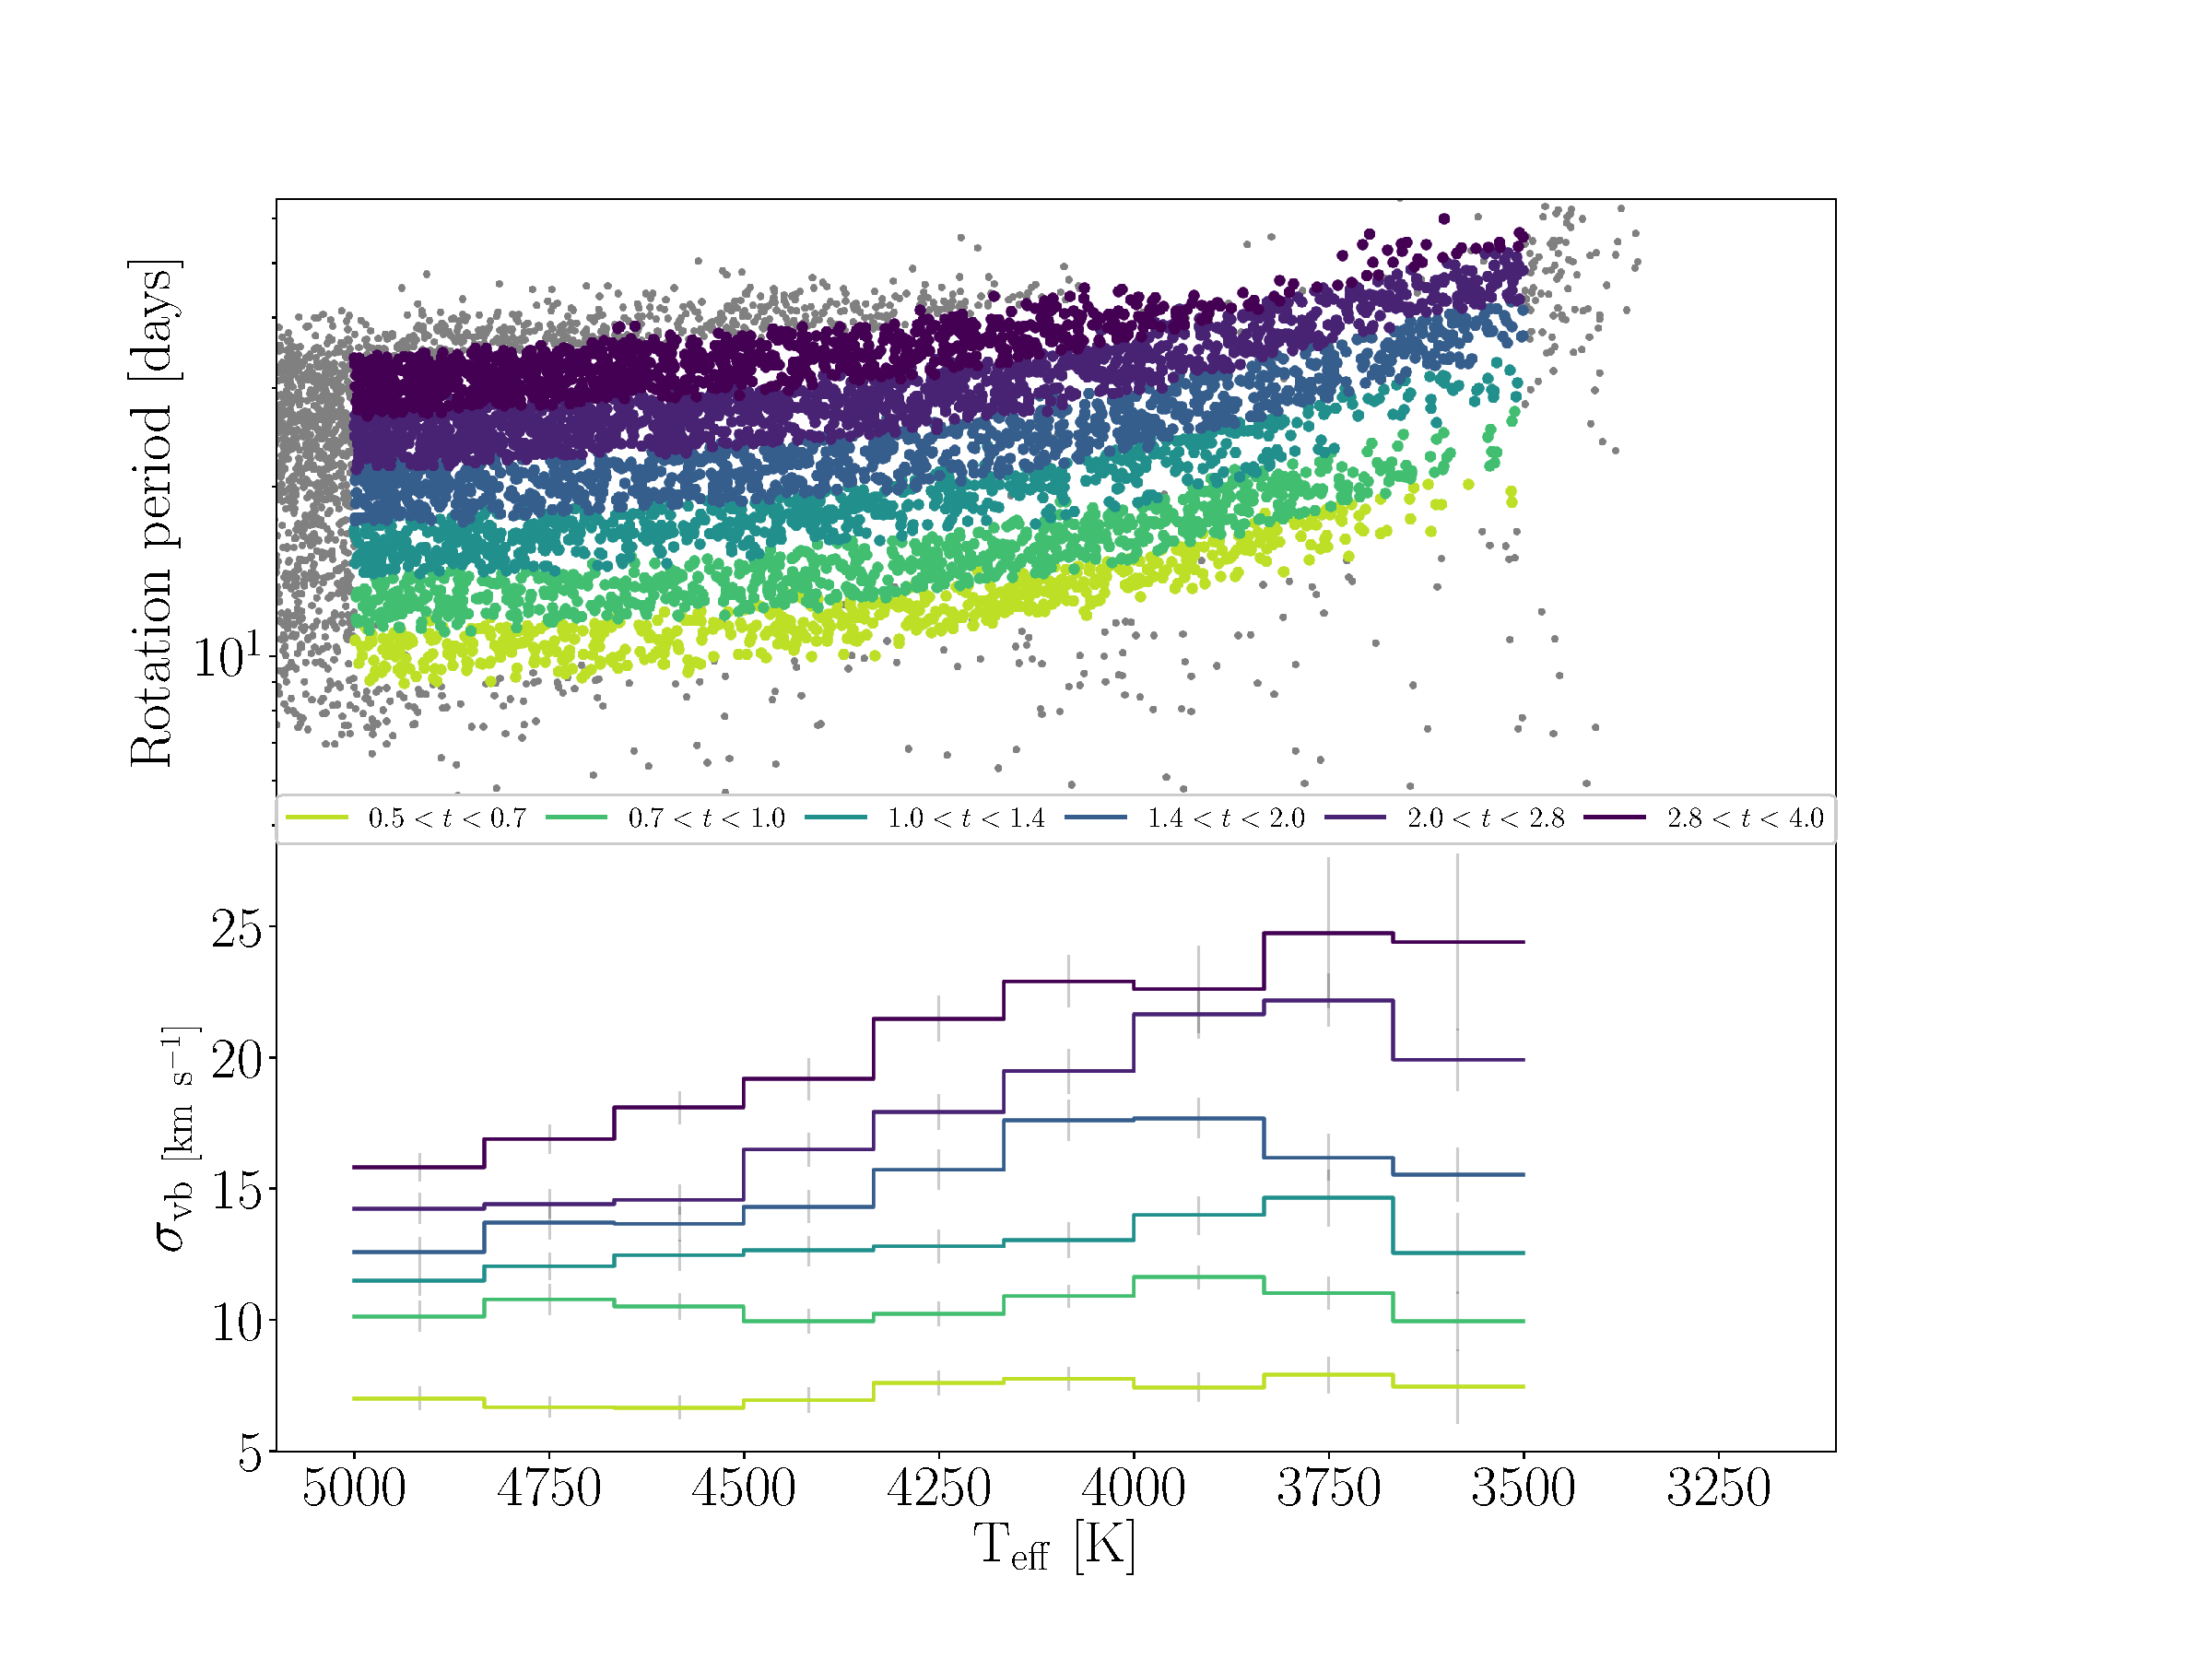
\includegraphics[width=1\textwidth]{age_cut}
\label{fig:age_cut}
\end{figure}
The top panel of figure \ref{fig:age_cut} shows the full \mct\ sample
(excluding visual binaries and subgiants) in grey, with coeval groups shown in
color.
The color of the points corresponds to the age ranges specified in the legend
(in Gyr), which also apply to the lines in the lower panel.
The bottom panel shows the velocity dispersion, \sigmavb\ of each age group,
as a function of effective temperature.
% We only included stars within a temperature range of 5000 - 3500 K in our
% analysis, as hotter stars are more likely to have stopped magnetic braking
% \citep{vansaders2016}, which could bias the results.
Late M dwarfs were not included in our analysis because such faint stars
cannot be observed at large heights above the plane (because of the low
galactic latitude of the \kepler\ field, stars at high-Z are more distant),
which introduces a mass-dependent velocity bias: cooler populations of stars
are skewed towards lower velocity dispersions.
The coolest temperature bins in the lower panel of figure \ref{fig:age_cut}
have low velocity dispersions, indicating that this effect may already become
important at temperatures lower than $\sim$ 4000 K.

Overall, figure \ref{fig:age_cut} shows that velocity dispersion increases
with gyrochronal age across all temperatures, implying that both velocity
dispersion and rotation periods increase with age as expected.
The constant velocity dispersion of young stars as a function of temperature
shows that the Praesepe-calibrated gyrochronology relation accurately predicts
the relative ages of {\it young} field stars.
% To our knowledge, no gyrochronology relation has never been demonstrated to
% correctly predict ages (either relative or absolute) for such cool or such
% young field stars.
% This is not particularly remarkable however, since these young stars are a
% similar age to the Praesepe cluster, which was used to calibrate the
% period-color relation.
% However, if the stars in each selected age group had the {\it same} age across
% the temperature range, their velocity dispersion would be a constant function
% of \teff.
In contrast however, velocity dispersion increases as a function of
temperature for old stars, meaning the \citet{angus2019} gyrochronology
relation underpredicts the ages of old, late-K dwarfs (or overpredicts the
ages of old early-K dwarfs).
This indicates that the relationship between period and photometric
color or \teff\ flattens out over time.
In other words, the lines of constant age sweeping diagonally upwards in the
top panel of figure \ref{fig:age_cut} are too steeply sloped at old ages.

\subsection{Mass-dependent heating}

An alternative explanation for this phenomenon is that lower-mass stars
experience greater velocity changes when gravitationally perturbed and are
more efficiently dynamically heated.
Mass-dependent orbital heating has not been unambiguously observed in the
galactic disk because of the strong anti-correlation between stellar mass and
stellar age.
Less massive stars do indeed have larger velocity dispersions, however they
are also older on average.
This mass-age degeneracy is highly reduced in M dwarfs because their
main-sequence lifetimes are longer than the age of the Universe, however no
evidence for mass-dependent heating has been detected in these low mass stars
\citep{faherty2009}.
To investigate further, we selected late K and M dwarfs observed by both
\kepler\ and \gaia, whose MS lifetimes exceed around 11 Gyrs and are therefore
representative of the initial mass function.
% This allowed us to remove the degeneracy between mass and age that would
% confound evidence for mass-dependent heating among more massive stars.
% In a sample of massive stars with short MS lifetimes, lower-mass stars
% typically have greater velocity dispersion, but this could be either because
% dynamical heating is more efficient in lower mass stars, or because lower mass
% stars tend to be older because they live longer.
% In a sample of late K and M dwarfs, whose MS lifetime is longer than the age
% of the Universe, we can assume that none have evolved into giants and any
% additional heating seen in the lower-mass stars must be caused by
% mass-dependent heating.
We selected all \kepler\ targets with dereddened \gaia\ \gcolor\ colors
greater than 1.2 (corresponding to an effective temperature $\lesssim$
4800 K) and absolute \gaia\ $G$-band magnitudes $<$ 4.
We also eliminated visual binaries by removing stars above a 6th order
polynomial, fit to the MS on the \gaia\ CMD.
% shown in figure \ref{fig:mdwarf_CMD}.
We then applied the same quality cuts as described in section
\ref{sec:the_data}.
% \begin{figure}
%   \caption{
% A \gaia\ color-magnitude diagram, showing all \kepler\ targets.
% We selected K and M dwarfs by applying color and magnitude cuts at \gcolor\ =
%     1.2 (\teff\ $\sim$ 4800 K) and $G$ = 4.
% We eliminated visual binaries by fitting a 6th order polynomial to the MS and
%     removing stars above it.
% Selected K and M dwarfs are shown as darker points.
% }
%   \centering
%     \includegraphics[width=1\textwidth]{mdwarf_CMD}
% \label{fig:mdwarf_CMD}
% \end{figure}
To search for evidence of mass-dependent heating we calculated the (\vb)
velocity dispersion of stars in effective temperature bins.
Again, we applied sigma clipping to remove high velocity outliers before
calculating the standard deviation of stars in each bin.
% A slight excess of non-Gaussian outliers at lower temperatures leads to a
% marginal increase in velocity dispersion at low temperatures when sigma
% clipping is not performed.
% Figure \ref{fig:vb_vs_color} shows velocity and velocity dispersion as a
% function of \gaia\ \gcolor\ color.
% There is no clear trend between velocity dispersion and color.
Figure \ref{fig:vb_vs_teff} shows velocity and velocity dispersion
as a function of effective temperature (calculated by transforming dereddened
\gaia\ colors using equation \ref{eq:curtis}).
Velocity dispersion very slightly {\it decreases} with decreasing temperature,
(the opposite of the trend expected for mass-dependent heating) however the
slope is only inconsistent with zero at the 1.3 $\sigma$ level.
This trend may be due to a selection bias: cooler stars are fainter and
therefore typically closer, with smaller heights above the galactic plane and
smaller velocities.
The essential point here is that the increasing velocity dispersion with age
and decreasing temperature that is evident in figure \ref{fig:age_cut} is not
a result of an intrinsically larger velocity dispersion for low-mass stars,
nor is it a result of the selection function.
Since we use \vb, not \vz\ in this analysis, it is possible that the
anti-correlation between \teff\ and galactic latitude, $b$, could influence
these results: stars at higher latitudes would have additional velocity
components in the ${\bf x}$ and ${\bf y}$ directions, which could increase
\vb\ but not \vz.
However, since the relationship between \sigmavb\ and \teff\ is positively,
not negatively correlated for cool stars in the \kepler\ field, this effect is
probably too small to influence our results.
We performed the same analysis on the 537 stars in this sample with RVs using
{\it vertical} velocity (\vz) and found the slope of the velocity
dispersion-temperature relation was consistent with zero.
% \begin{figure}
%   \caption{
%       Top: Stellar velocity (\vb) as a function of \gaia\ \gcolor\ color for
%       \kepler\ K and M dwarfs.
% Vertical lines indicate different color-groupings used to calculate velocity
%     dispersion.
% Pink stars were not included in velocity dispersion calculations as they were
%     removed as outliers during a sigma clipping process.
% Bottom: velocity dispersion as a function of color.
% There is no obvious trend between velocity dispersion and stellar color
%     indicating that mass-dependent heating does not significantly effect
%     low-mass stars in the \kepler\ field.
% }
%   \centering
%     \includegraphics[width=1\textwidth]{vb_vs_color}
% \label{fig:vb_vs_color}
% \end{figure}

\begin{figure}
  \caption{
      Top: Stellar velocity (\vb) as a function of \teff\ for
      \kepler\ K and M dwarfs.
Vertical lines indicate different \teff-groupings used to calculate velocity
    dispersion.
Pink stars were not included in velocity dispersion calculations as they were
    either removed as outliers during a sigma clipping process, or they lie at
    the sparcely populated, extremely cool end of the temperature range.
    Velocity dispersion and \teff\ are slightly positively correlated, likely
    due to a brightness-related selection bias, indicating that mass-dependent
    heating does not significantly affect low-mass stars in the \kepler\
    field.
}
  \centering
    \includegraphics[width=1\textwidth]{vb_vs_teff}
\label{fig:vb_vs_teff}
\end{figure}
Figure \ref{fig:vb_vs_teff} indicates that mass-dependent heating does not
strongly affect the \mct\ sample of rotating \kepler\ stars.
For this reason, we assume that age difference is the only significant cause
of velocity dispersion differences between groups.
In other words, (\vb) velocity dispersion is a reliable age proxy for the
\mct\ sample.

% The \vb\ AVR is not directly comparable to the \vz\ AVR, so, to draw a
% comparison with results from the literature, we calculated a \vz\ AVR for
% the subset of 290 cool stars in the \mct\ sample with \gaia\ RVs.
% We measured an AVR exponent of 0.47 $\pm$ 0.1, which falls within the range of
% values (0.45-0.53) reported from measurements of F and G stars in the Solar
% neighborhood \citep{holmberg2009, aumer2009, aumer2016}.
% It is a little lower than the values of 0.56 $\pm$ 0.14 (for low-z) and 0.51
% $\pm$ 0.15 (for high-z stars), calculated using \LAMOST\ \racomment{(LAMOST
% citation)} K giants \citep{yu2018}.
% K giants are more massive than K dwarfs \racomment{(how much more massive?)},
% so this slightly higher value contradicts the mass-dependent heating
% hypothesis.
% \racomment{Add some words about selection functions...}

% To investigate further, we calculated the exponent of the (\vb) AVR for each
% temperature bin in figure \ref{fig:age_cut}.
% \begin{figure}
%   \caption{
%       The exponent of the (\vb) AVR as a function of effective temperature.
% }
%   \centering
%     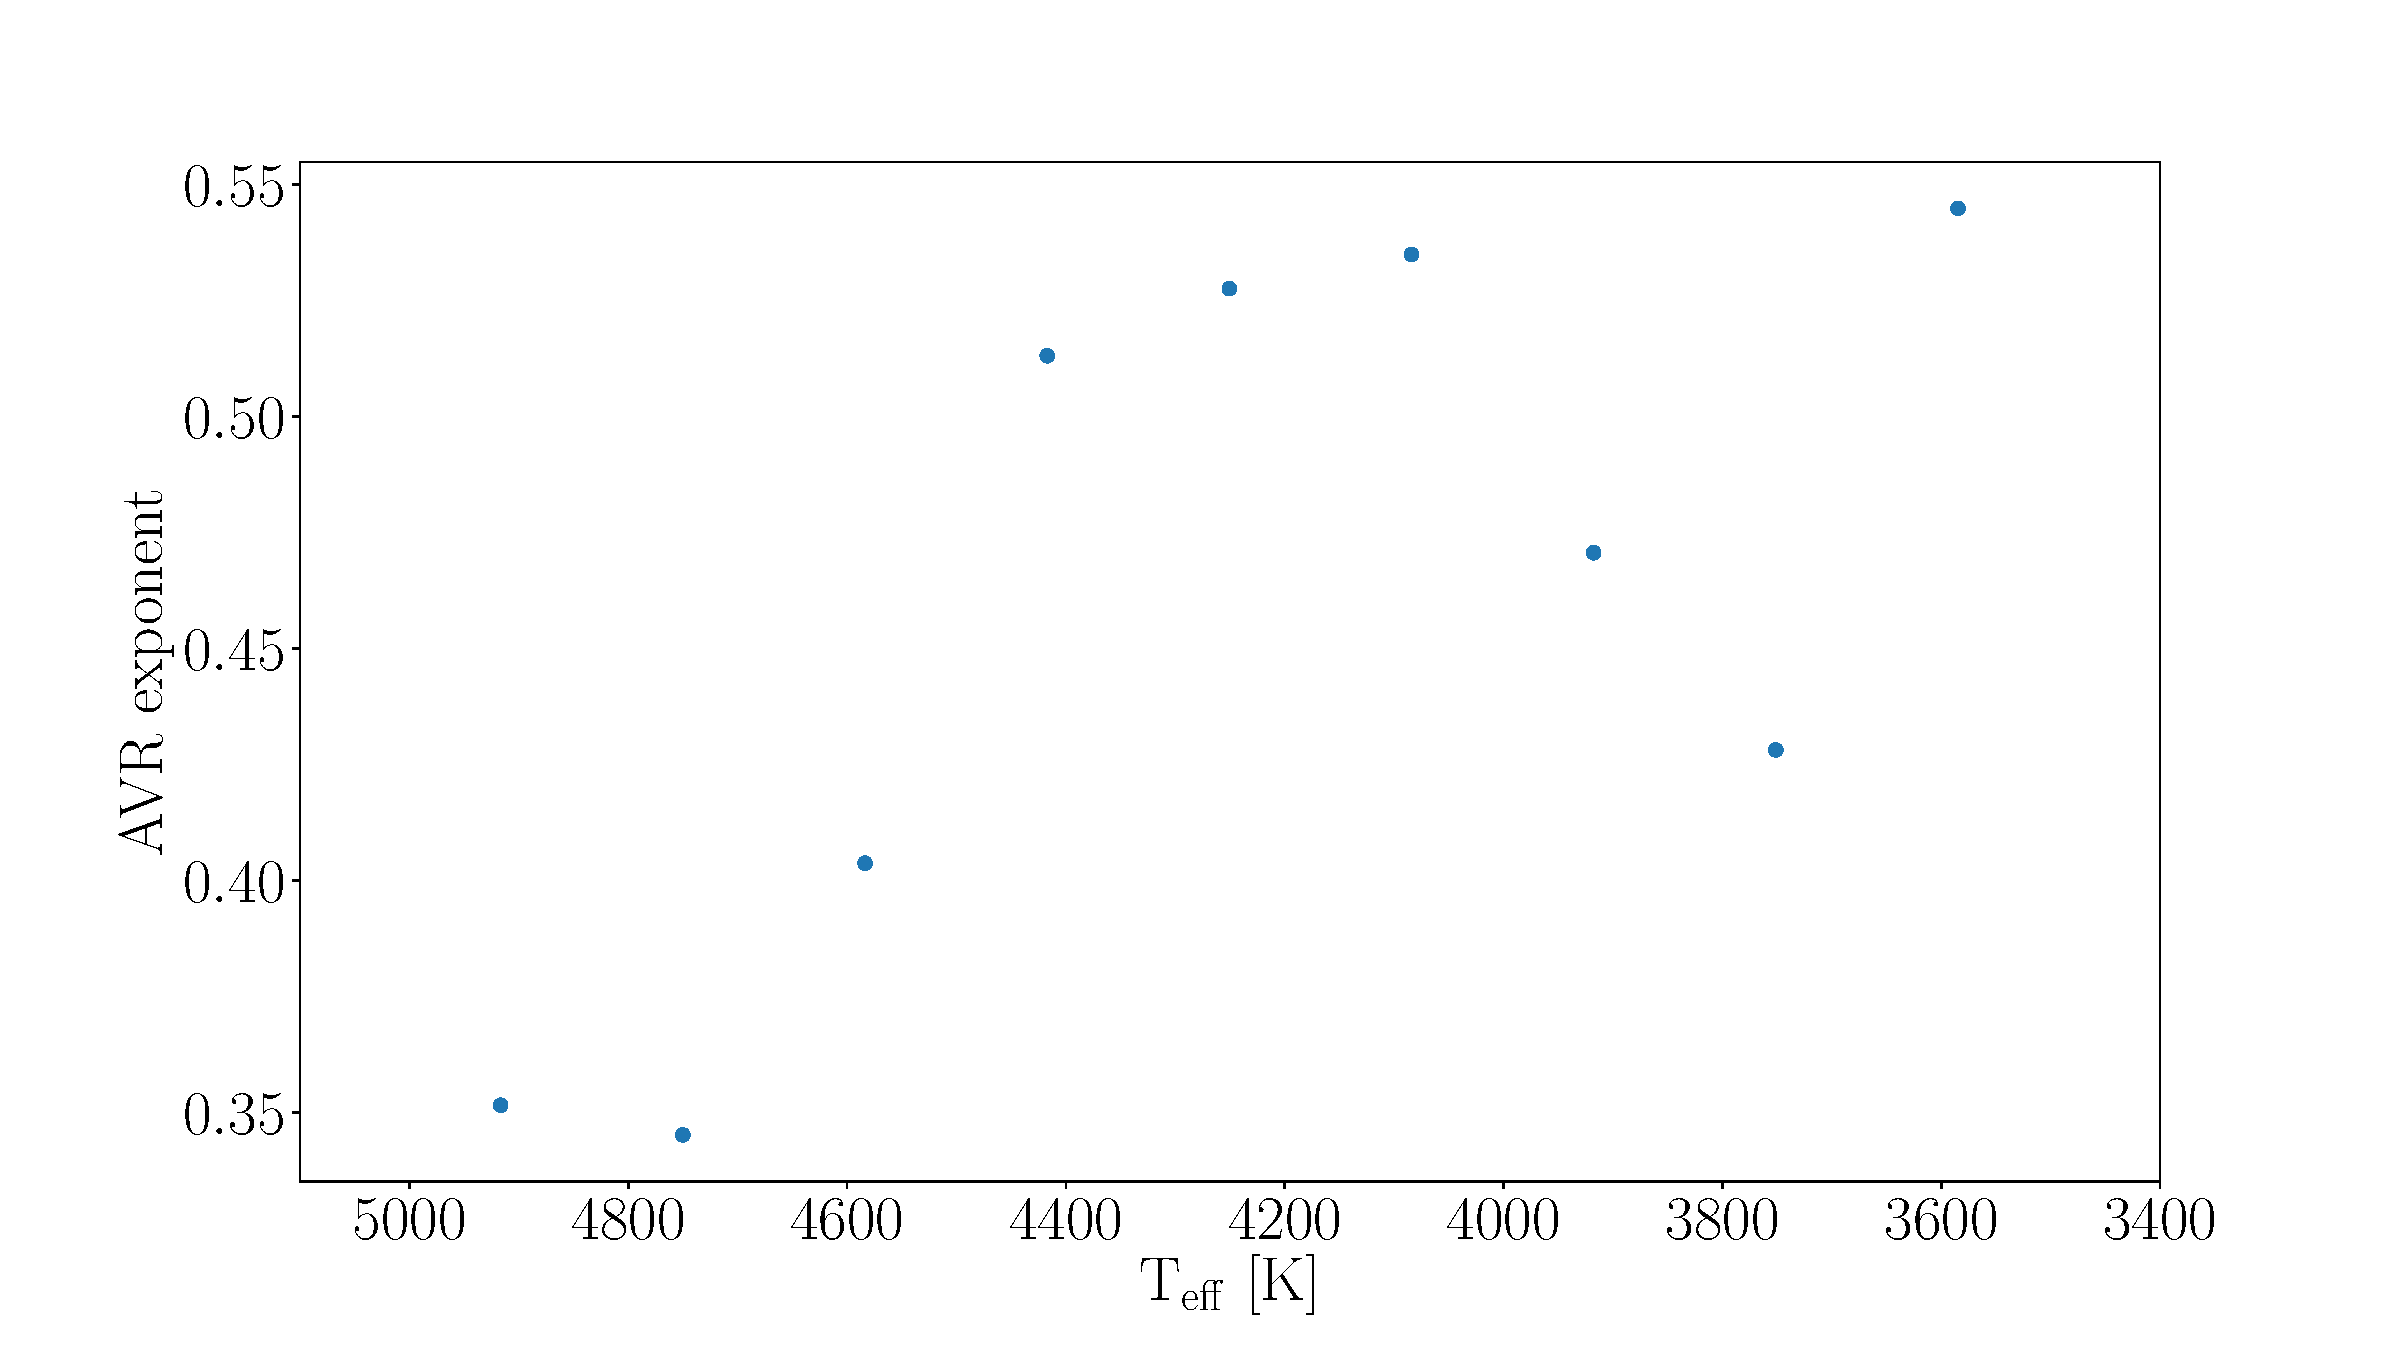
\includegraphics[width=1\textwidth]{AVR_exponent}
% \label{fig:AVR_exponent}
% \end{figure}
% Figure \ref{fig:AVR_exponent} shows the significant rise the in AVR exponent
% as a function of effective temperature.
% The hottest stars in our sample (\teff\ = 4833-5000 K) have a (\vb) AVR
% exponent of 0.39 $\pm$ 0.02 and the coolest (\teff\ = 3500-3667 K) have an
% exponent of 0.74 $\pm$ 0.02.
% The masses of stars in our sample differ by less than a factor of two,
% so mass-dependent heating cannot be entirely responsible for this large spread
% in heating rates.
% \racomment{Need to look into this further.}

% If mass-dependent heating is strongly affecting our data, the exponent of the
% AVR should increase with decreasing effective temperature, \ie\ the heating
% rate should be greater for lower-mass stars.
% Figure \ref{fig:AVR_exponent} shows the AVR exponent does indeed increase with
% decreasing effective temperature, however, the AVR exponent calculated using
% more massive stars from the Geneva Copenhagen Survey (GCS)
% \citep{holmberg2009} is also shown on this plot as a dashed horizontal line.
% Most GCS stars are F and G type: 1-3 times more massive than the K dwarfs used
% in our study.
% If mass-dependent orbital heating is the main cause the rise in velocity
% dispersion with decreasing \teff\ seen in figure \ref{fig:age_cut}, then the
% AVR exponent of the more massive GCS stars should fall {\it below} the AVR
% exponent for the most massive stars in our sample.
% In other words, the dynamical heating rate should be lowest for the highest
% mass stars and highest for the lowest mass stars.
% % nordstrom2004, jorgensen2005,
% These AVR exponents were calculated with different populations of stars,
% subject to different selection effects, so directly comparing them comes with
% some risk.
% The most important difference is that the GCS AVR is calculated using \vz,
% however our AVRs are calculated using \vb\ since most stars in our sample do
% not have radial velocities.
% The median galactic latitude of these \kepler\ stars is 12.3\degrees, with
% latitudes ranging from 5.5\degrees\ to 21.4\degrees, so \vb\ is a relatively
% close approximation to \vz.
% Only 290 out of the 6820 stars in our sample, plotted in color in figure
% \ref{fig:age_cut}, have \gaia\ radial velocities, however we used the ones
% that do to compare the \vz\ AVR to the \vb\ AVR, across all temperatures
% between 3500 and 5000 K.
% For stars with gyrochronal ages between 0.5 and 4.5 Gyr, we measured a \vz\
% AVR exponent of 0.519 $\pm$ ... and a \vb\ AVR exponent of 0.514 $\pm$... .
% The similarity of these two AVR exponents suggests that directly comparing
% these two quantities {\it may} be a reasonable approach.
% For now, given the large difference between the (\vz) AVR exponent of the GCS
% sample and the (\vb) AVR exponent of the hottest stars in our sample, we
% assume that the increased velocity dispersion at cooler temperatures is mostly
% caused by incorrect age-grouping due to an incorrect period-color relation at
% old ages, and that any mass-dependent heating, while it may contribute at a
% low level to this result, is not the dominant driver.
% However, differentiating the effects of mass-dependent heating and the shape
% of the gyrochronology relations is certainly warranted in a follow-up study.
% }

% Figure \ref{fig:age_comparison} shows the ages of star groups, predicted with
% the \citet{angus2019} gyrochronology relation, compared with the ages of star
% groups, predicted with the \citet{holmberg2009} AVR.
% \citet{holmberg2009} only provide an exponent (0.53), not an intercept, for the
% relation between logarithmic age (in Gyr) and logarithmic, \vz\ velocity
% dispersion (in \kms), so we fit the intercept to the mean \vb\ velocity
% dispersion across all temperatures, of our sample.
% \begin{figure}
%   \caption{
%       Ages predicted by the \citet{holmberg2009} \vz\ AVR, against ages
%     predicted by the \citet{angus2019} gyrochronology relation, for stars in
%     different temperature ranges.
% Points are colored by the effective temperature in the center of the \teff\
% bin.
% The dashed line shows the y=x relation.
% Predicted kinematic ages fan out over gyrochronal time, either because the AVR
%     is temperature-dependent or because the gyrochronology relations have an
%     age-dependent period-color relation.
% }
%   \centering
%     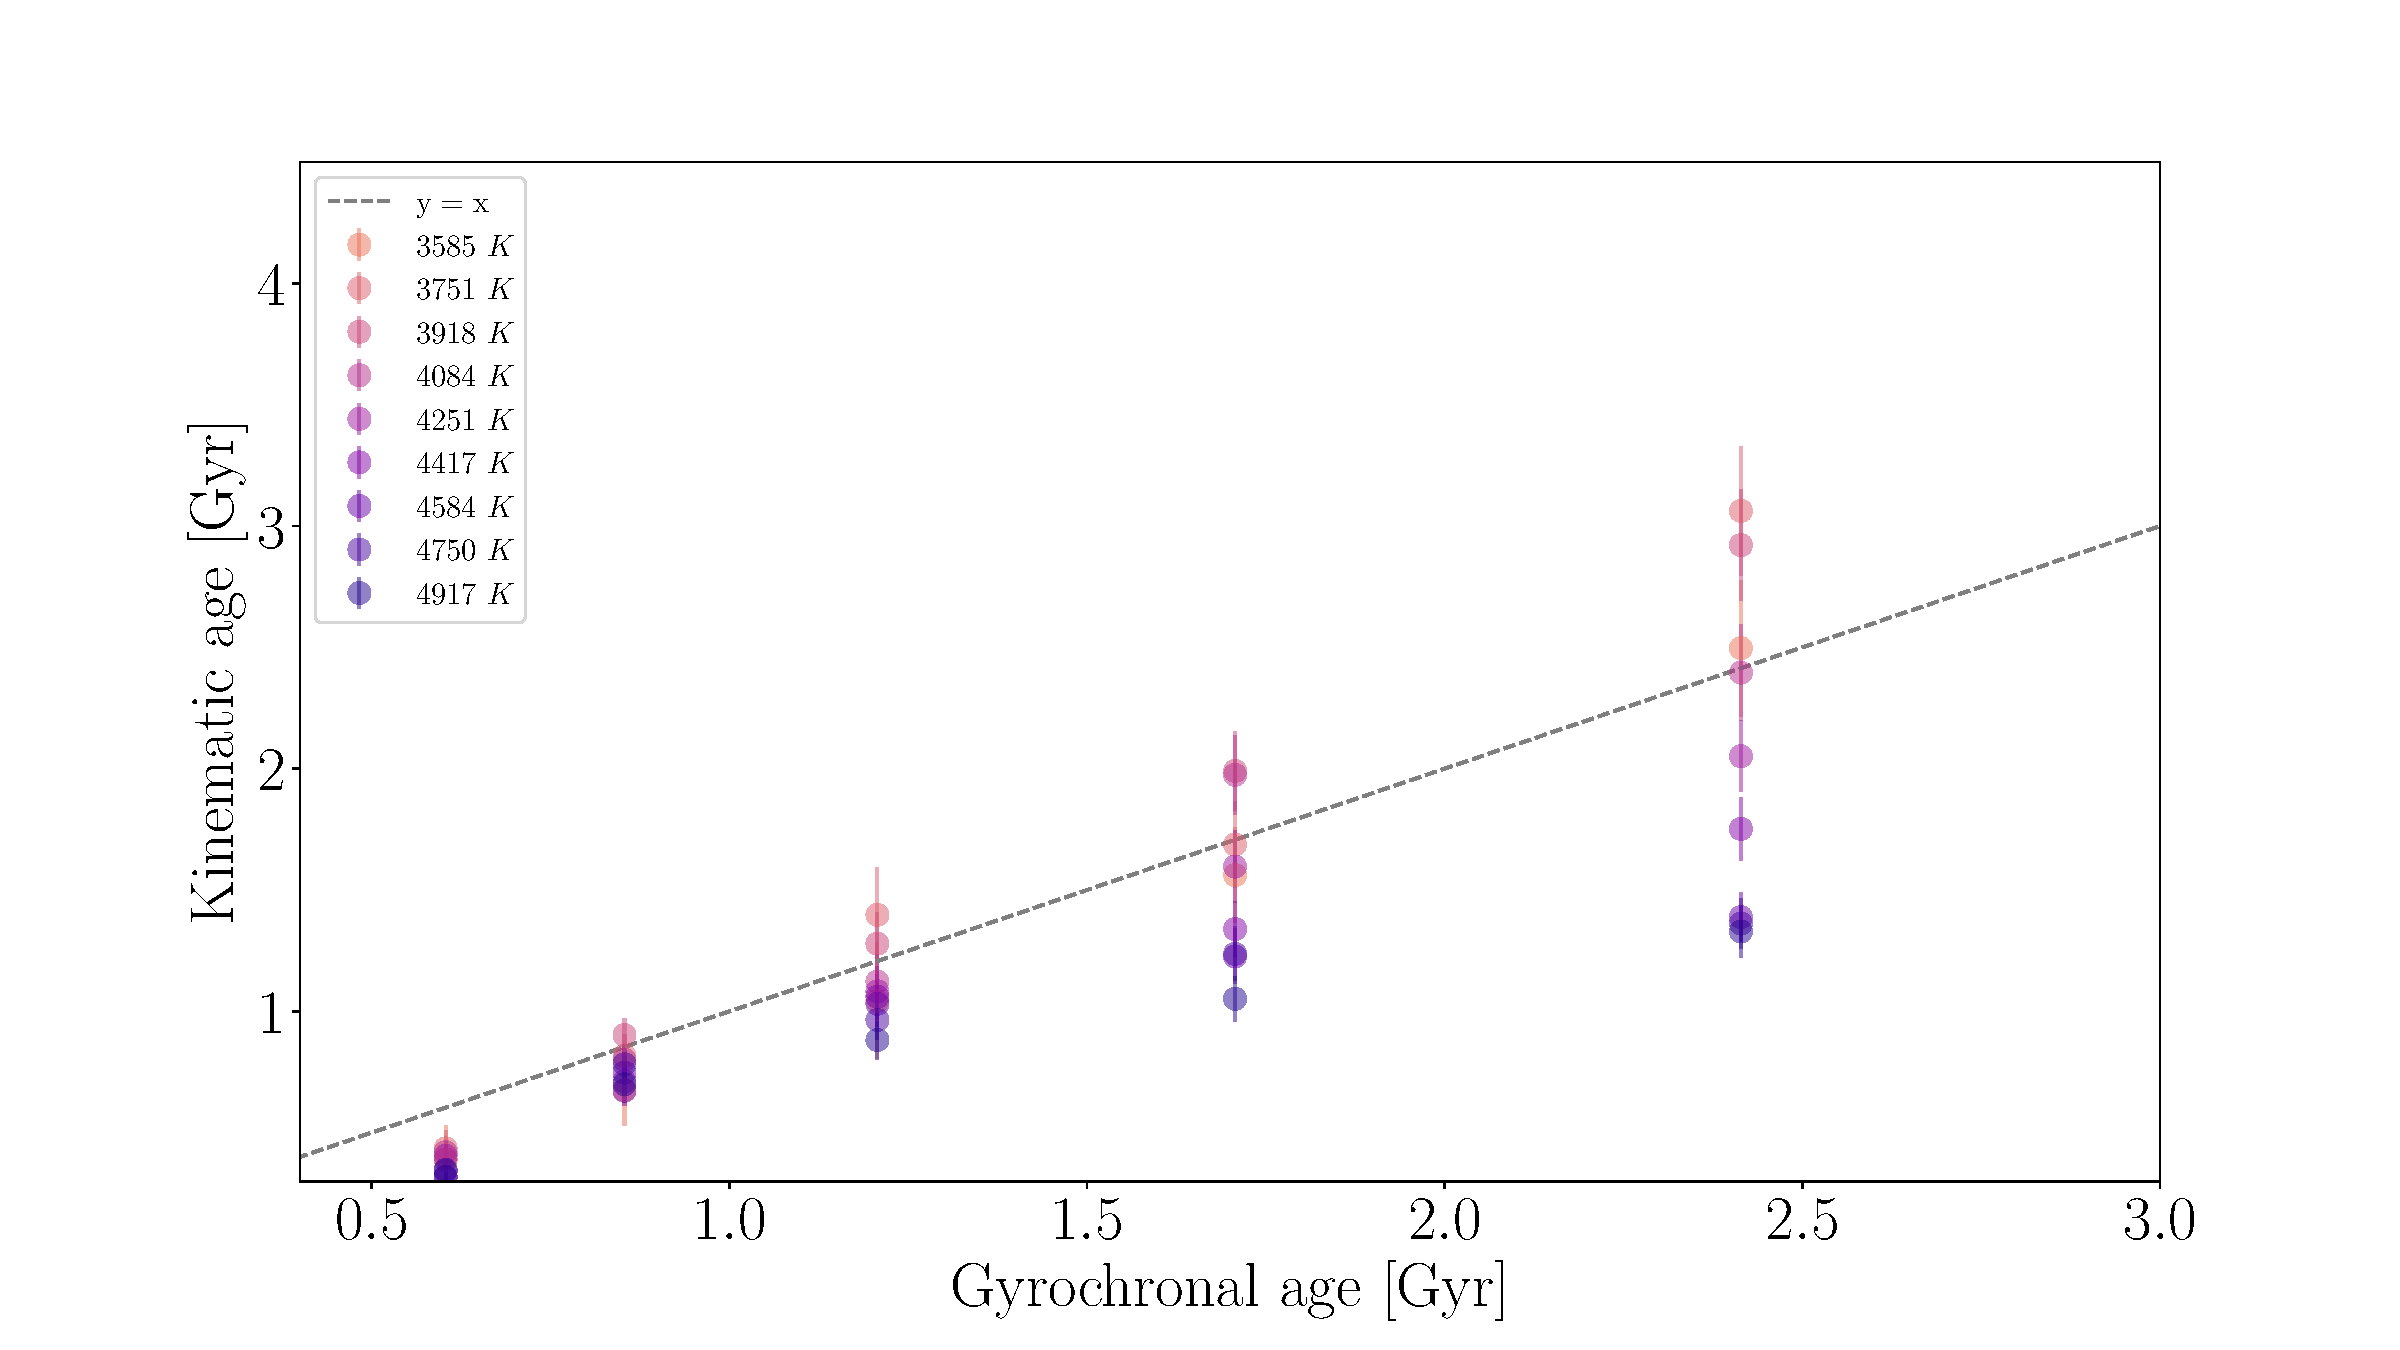
\includegraphics[width=1\textwidth]{age_comparison}
% \label{fig:age_comparison}
% \end{figure}
% Figure \ref{fig:age_comparison} shows a comparison between ages predicted by
% the \citet{holmberg2009} \vz\ AVR (using \vb\ as a proxy for \vz) and ages
% predicted by the \citet{angus2019} gyrochronology relation, for stars in
% different temperature ranges.
% The predicted kinematic ages fan out over gyrochronal time, either because the
% AVR is temperature-dependent or because the gyrochronology relations have an
% age-dependent period-color relation.
% Figure \ref{fig:age_comparion} also suggests that dynamical heating does not
% begin until after around ... Gyr:

% Alternatively, the ages of these young stars could be under-predicted by
% gyrochronology.
% These young stars have similar rotation periods to the Praesepe cluster, which
% was used to calibrate the gyrochronology relation used in this analysis.
% The ages of these young stars should, therefore, be the most accurate of the
% entire sample.
% However, they are tied to the age of the Praesepe cluster, whose age is not
% accurately known.
% \citet{angus2019} adopted an age for Praesepe of 650 Myrs, however the
% kinematic age-prediction for these stars is around 400 Myrs.
% Other studies have assigned a much older age of 800 Myrs to Praesepe
% \citep{brandt2015}.
% If the age assumed for Praesepe in the \citet{angus2019} gyrochronology
% calibration was inaccurate, the entire age {\it scale} would be incorrect.
% However, this is not what figure \ref{fig:age_comparion} shows -- it shows
% that the {\it relative} age of these youngest stars are under-predicted by
% kinematics or over-predicted by gyrochronology.

% If we assume that the rise in velocity dispersions at cooler effective
% temperatures is caused by an inaccurate period-color relation rather than
% mass-dependent dynamical heating, we can estimate what the shape of the
% period-color relations {\it should} be.
% Figure \ref{fig:age_cut} indicates that the period-color relation flattens
% out, so we applied the same analysis to groups of stars with similar rotation
% periods, equivalent to a completely flat period-color relation.
% The top panel of figure \ref{fig:period_cut} shows the \mct\ sample with stars
% in different period ranges plotted in different colors.
% The bottom panel shows the velocity dispersion of each group as a function of
% effective temperature.
% \begin{figure}
%   \caption{
% This figure is similar to figure \ref{fig:age_cut}, with stars divided into
%     period groups rather than age groups.
% The velocity dispersion is more constant across effective temperatures for the
%     most slowly rotating stars, compared to the stars selected with the
%     \citet{angus2019} gyrochronology model, indicating that the gyrochronology
%     models flatten out, and possibly even invert, at old ages.
% }
%   \centering
%     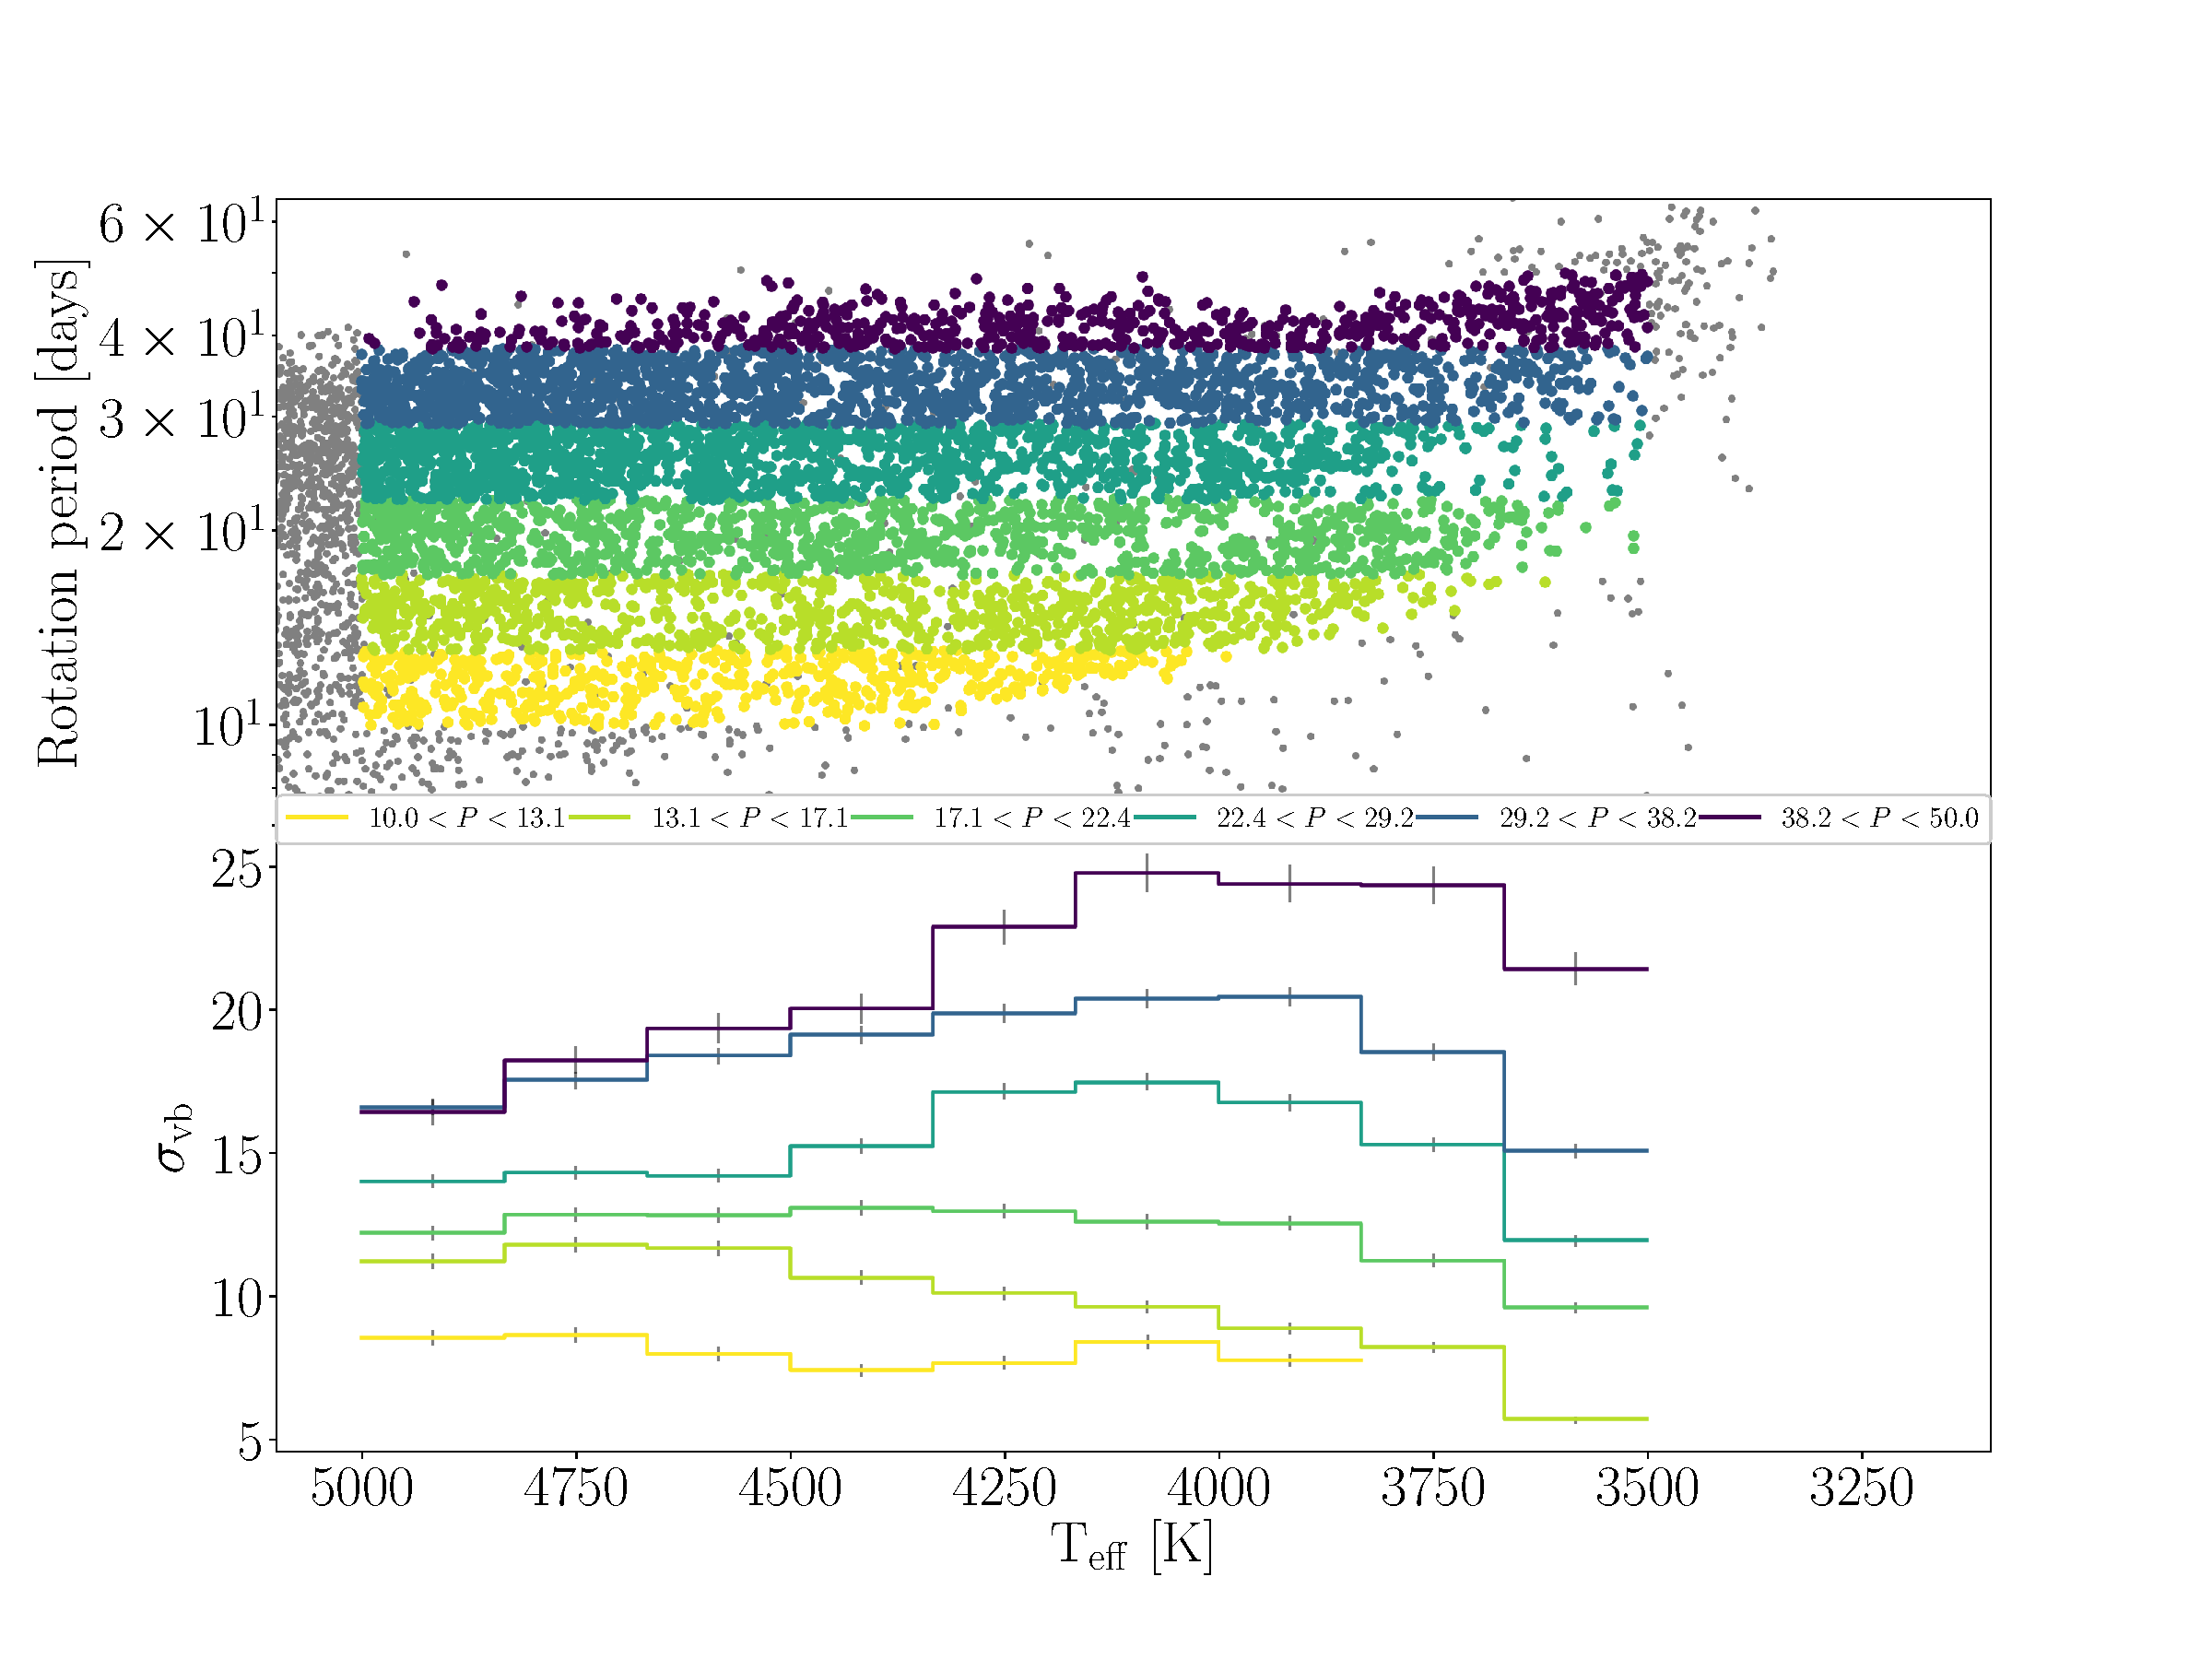
\includegraphics[width=1\textwidth]{period_cut}
% \label{fig:period_cut}
% \end{figure}
% Once again, the velocity dispersion increases with rotation period overall.
% For the most rapidly rotating groups of stars, velocity dispersion decreases
% with \teff\ as expected given the positively sloped period-color relation of
% Praesepe and other young clusters: late K dwarfs rotate more slowly than early
% K dwarfs of the same age.
% Between rotation periods of 15 and 25 days, the temperature dependence of the
% velocity dispersion starts to disappear, indicating that the period-color
% relation becomes flat: late K dwarfs rotate at the same rate as early K dwarfs
% of the same age.
% At long rotation periods, the velocity dispersion still increases with
% effective temperature, although the increase is much more modest compared to
% the oldest stars in figure \ref{fig:age_cut}.

% If we assume the rise in velocity dispersion at cooler effective temperatures
% is caused by an inaccurate period-color relation rather than mass-dependent
% dynamical heating, we can generate a graphical representation of what the
% relations {\it should} look like.

\subsection{The period-\teff\ relations, revealed}

\begin{figure}
  \caption{
Rotation period vs effective temperature for stars in the \mct\ sample,
    colored by the velocity dispersions of stars in restricted period and
    temperature ranges.
}
  \centering
    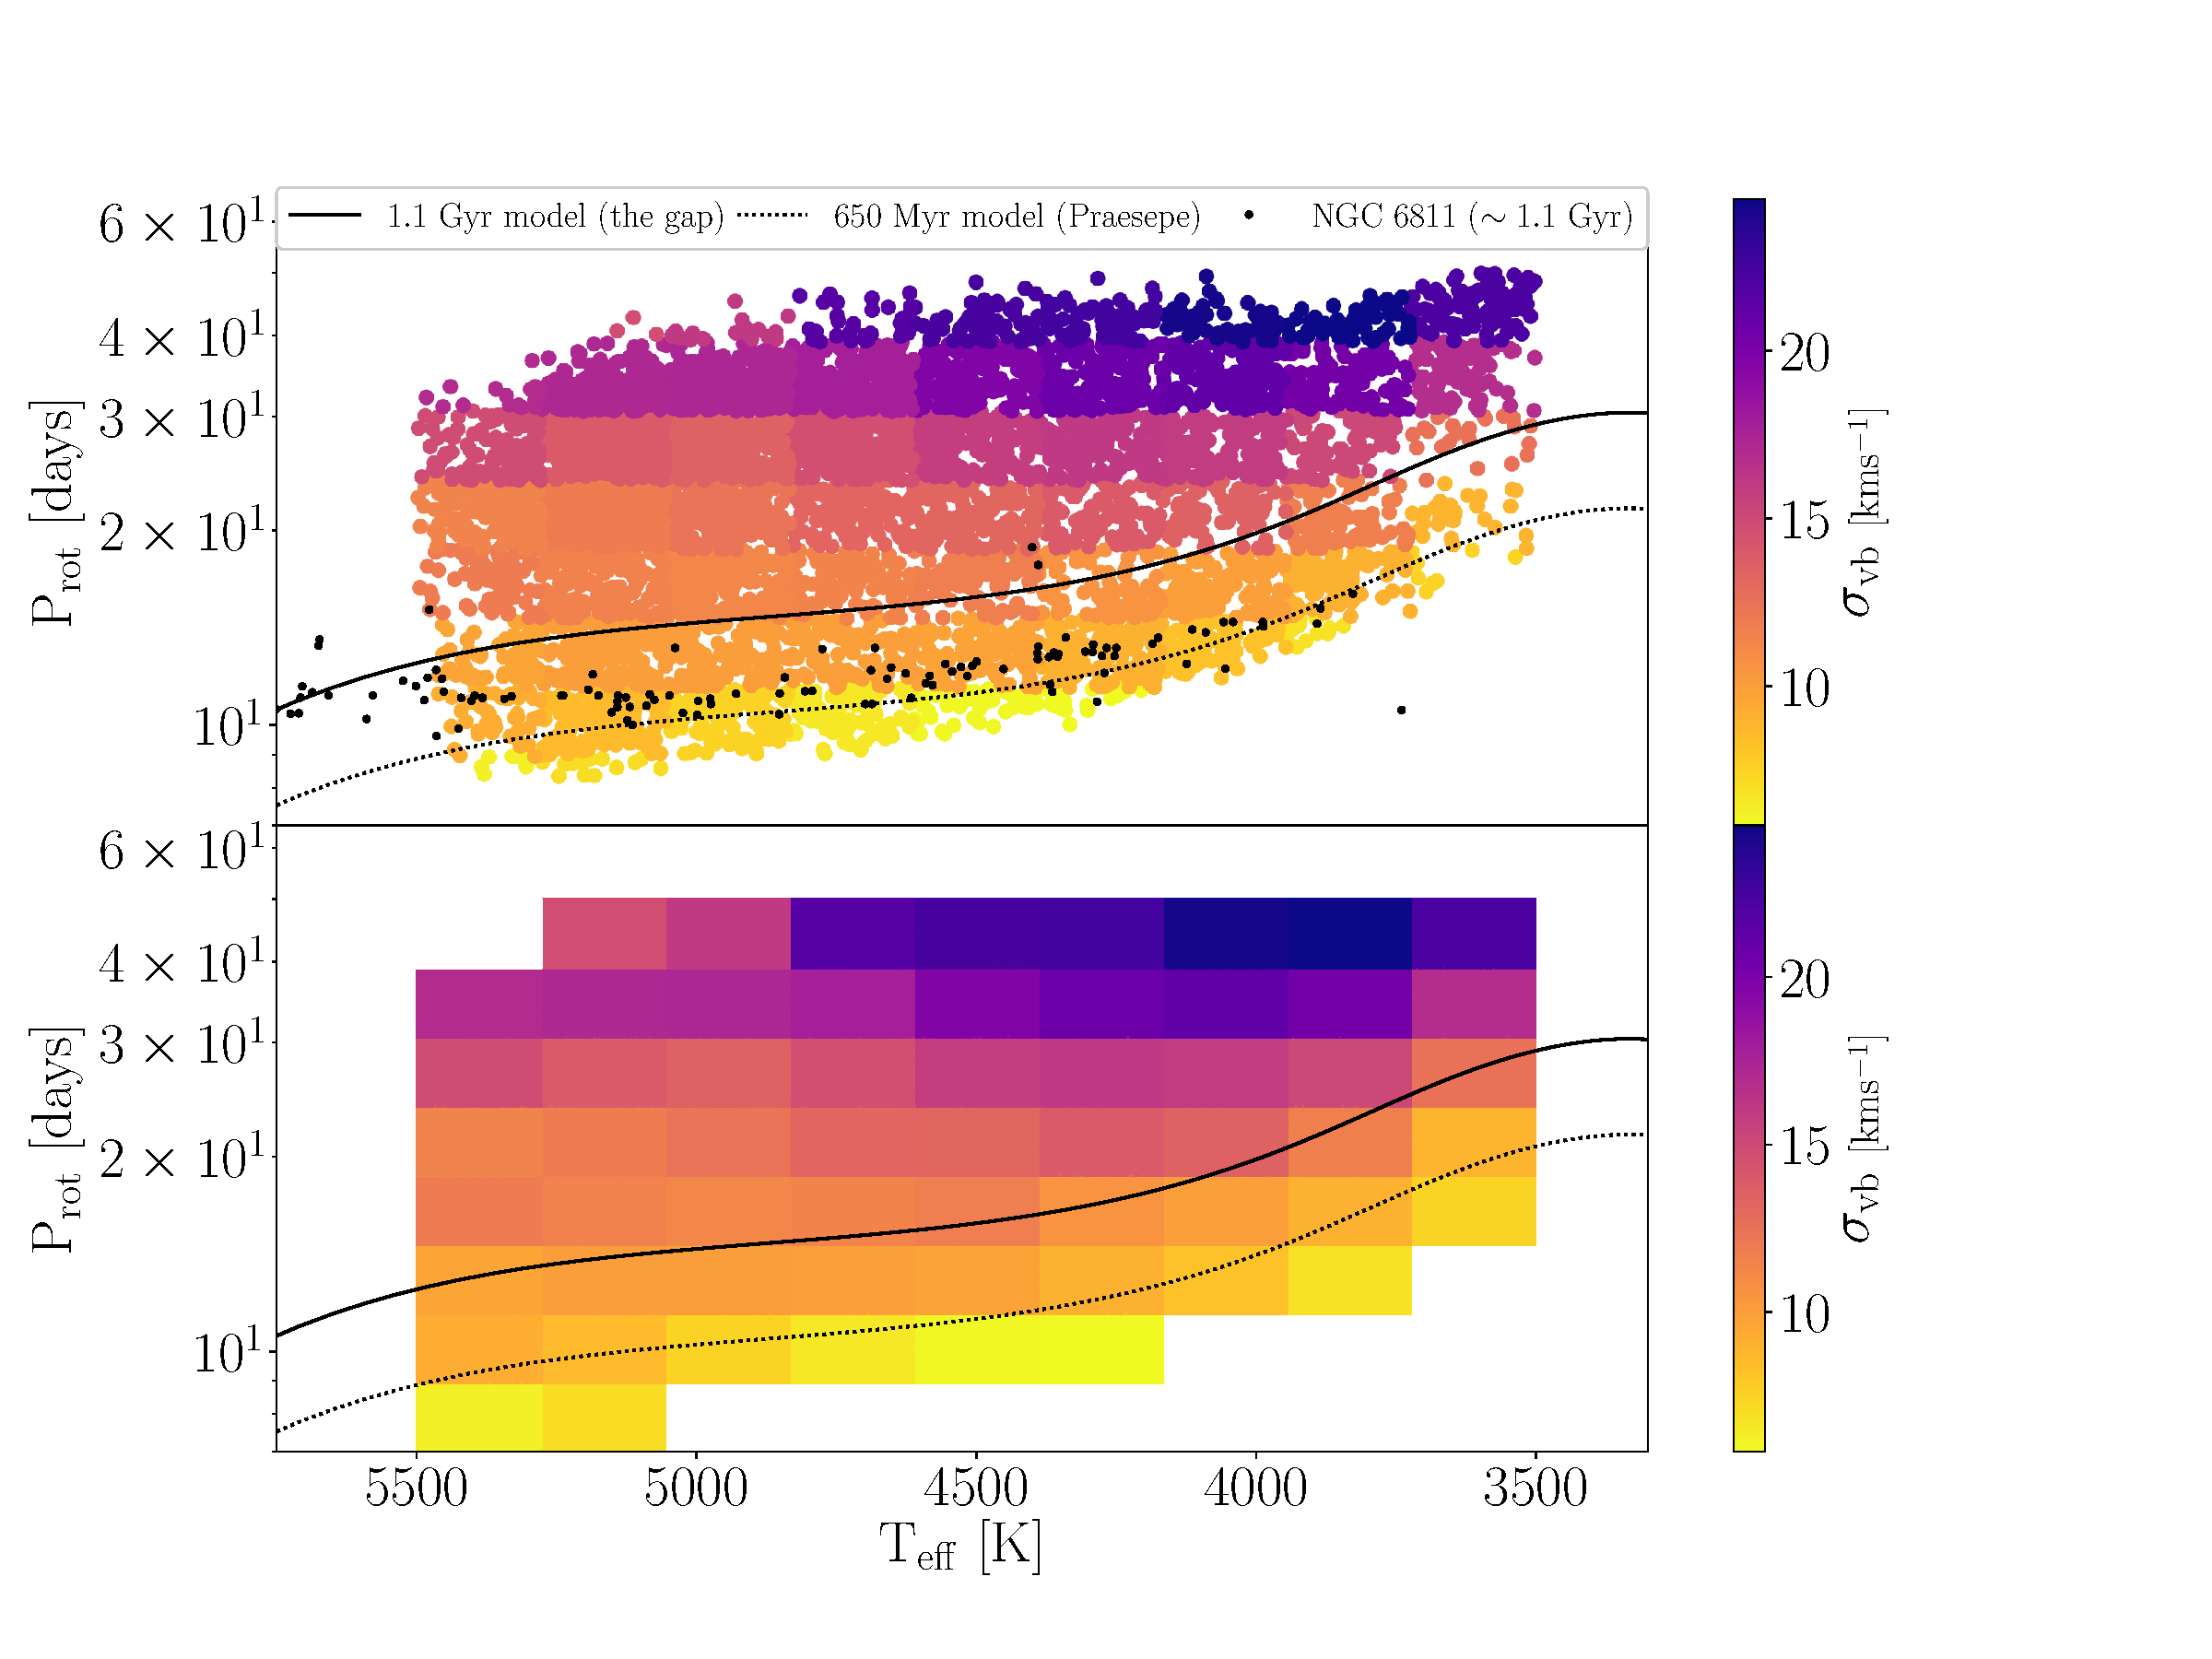
\includegraphics[width=1\textwidth]{vplot}
\label{fig:dispersion_period_teff}
\end{figure}
Figure \ref{fig:dispersion_period_teff} shows rotation period vs. \teff\ for
our sample, coloured by (\vb) velocity dispersion.
Here, velocity dispersion was calculated for groups of stars in
uniformly-spaced bins in $\log_{10}$(period) and temperature.
If we assume that mass dependent heating doesn't affect this sample, and \vb\
at low galactic latitudes is an unbiased tracer of \vz, \vb\ velocity
dispersion can be interpreted as an age proxy and stars plotted in a similar
color in figure \ref{fig:dispersion_period_teff} are similar ages.
Interpreted this way, it appears that rotation period {\it decreases} with
decreasing effective temperature at old ages.  This is a paradigm shift
for gyrochronology because stellar spin-down rate is thought to be directly
tied to magnetic field strength, and the deeper convection zones of cooler
stars generate stronger magnetic fields which {\it should} lead to more
efficient angular momentum loss.
A similar phenomenon has been observed in the 1.1 Gyr NGC 6811 cluster, where
the rotation periods of mid-K dwarfs are faster than expected; their
rotational evolution appears to have stalled, and the period-\teff\ relation
is flat \citep{curtis2019}.
NGC 6811 straddles the rotation period gap and may be the `missing link' that
connects two epoch of stellar spin-down: an early stage where the
period-\teff\ relation for K dwarfs has a negative slope and a late stage
where it has a positive slope.
In this case the period gap may delineate the transition between these two
regimes and is the point at which stellar magnetic dynamos likely undergo a
dramatic structural shift.

Figure \ref{fig:dispersion_period_teff} also shows that the (kinematically)
oldest stars with measured rotation periods are cooler than 4500 K.
This may be because cooler stars remain active for longer, and their rotation
periods can therefore be measured at older ages.

% Unfortunately, we still cannot rule out the possibility that mass-dependent
% heating is acting on these stars which could be responsible for some, if not
% all, of the increased velocity dispersion at cooler effective temperatures.

\subsection{The period gap}
An unsolved mystery within gyrochronology is the origin of the rotation period
gap, first identified by \citet{mcquillan2013}.
This gap can be seen in figure \ref{fig:age_cut} as an under-density of points
between the 0.7-1.0 and 1.0-1.5 Gyr age ranges and roughly follows a line of
constant gyrochronal age of around 1.1 Gyr \citep[according to
the gyrochronology relation of][]{angus2019}.
Several explanations for its origin have been proposed, including a
discontinuous star formation history \citep{mcquillan2013, davenport2017,
davenport2018}, a rapid change in magnetic field structure
\citep{reinhold2019}, and erroneous rotation period measurements that are
incorrect by a factor of two \citep{koen2018}.
The latter explanation can be ruled out because stars below the gap have
smaller velocity dispersions than the stars above the gap, indicating that
they are kinematically younger \citep{mcquillan2013, davenport2018}, as
evident in figure \ref{fig:age_cut}.
For stars below the gap, in the 0.7-1.0 Gyr age range shown in figure
\ref{fig:age_cut}, velocity dispersion is relatively constant as a function of
temperature, however above the gap, in the 1.0-1.5 Gyr age range and older,
velocity dispersion increases with \teff.
The coolest stars in the 1.0-1.5 Gyr age range have the same velocity
dispersion as the hottest stars in the age range above which indicates that
the period-\teff\ relations are {\it flat} at these rotation periods.
It may be a coincidence that the gyrochronology relations seem to only flatten
off {\it above} the period gap, or it may be that the period gap is located at
magnetic transition period.
We lack a sufficient quantity of data to investigate in detail but new field
star rotation periods from the \ktwo\ and \tess\ missions may be able to
validate or rule out this hypothesis in the future.
